\section{System Overview}
\label{sec:fdsp-tpcelec-overview}

The main difference between the \dword{dune} \dword{sp} \dword{detmodule} %detector 
and 
previous experiments or prototypes using \dword{lar} technology is
that for the first time all the signal processing for the readout of the
wires of the \dwords{apa} takes place inside the the \dword{lar}, in boards that 
are directly mounted on the \dword{apa}. Accordingly, the \dword{tpc} 
readout electronics are referred to as the \dword{ce}. 

The electronics are 
mounted inside the \dword{lar} to exploit the fact that charge carrier 
mobility in silicon is higher, and %that 
thermal fluctuations are lower,  
at \dword{lar} temperature than at room temperature. For \dword{cmos} 
electronics, this results in substantially higher gain and lower noise 
at \dword{lar} temperature than at room temperature~\cite{DeGeronimo:2011zz}.
Mounting the \dword{fe} electronics on the \dword{apa} frames also minimizes 
the input capacitance, which also contributes to the noise reduction.  
Furthermore, placing the digitizing and multiplexing electronics inside 
the cryostat reduces the total number of penetrations into the cryostat 
and minimizes the number of cables coming out of it. %the cryostat.  

As the full \dword{tpc} electronics chain for the \dword{spmod} includes 
many components on the warm side of the cryostat as well, the \dword{dune} 
consortium designated to develop %organize development of 
this system is formally called 
the \dword{dune} \dword{sp} \dword{tpc} electronics consortium, but  %It is 
sometimes referred to as the \dword{ce} consortium. % for short.

%In this Section~\ref{sec:fdsp-tpcelec-overview} we 
This section starts with a review of the considerations that
have led to the proposed design for the \dword{dune} \dword{sp} detector, 
%followed by a discussion of 
then discusses how the detector requirements follow %are derived
from the physics goals of the experiment. %Later we demonstrate the validation of the design provided by the early data from the \dword{pdsp} prototype. 
Later we demonstrate how early data from \dword{pdsp} 
validates the design and  %We also 
discuss how the lessons learned from the construction,
integration, installation, and commissioning of \dword{pdsp} have 
informed the design changes that we are planning for the \dword{dune}
\dword{spmod}. % detector. 

%In the rest of this Chapter~\ref{ch:sp-tpcelec} we provide 
The reader will find a detailed
description of all the \dword{ce} detector components in Section
\ref{sec:fdsp-tpcelec-design}, followed by discussions of the \dword{qa}
program and %of 
the plans for production and assembly, and for integration,
installation and commissioning, in 
Sections~\ref{sec:fdsp-tpcelec-qa}--\ref{sec:fdsp-tpcelec-integration}. 
%Later, we discuss the interfaces with detector components provided by other consortia, with Technical Coordination, and with the Physics group, in Section~\ref{sec:fdsp-tpcelec-interfaces}. 
Section~\ref{sec:fdsp-tpcelec-interfaces} discusses the interfaces with detector components provided by other consortia, with \dword{tc}, and with the physics group. 
%This chapter concludes with a description of 
Sections~\ref{sec:fdsp-tpcelec-safety}--\ref{sec:fdsp-tpcelec-management} conclude the chapter with  plans for addressing safety issues and risks during the
construction, installation, and operation of the detector, and %with a discussion of 
an outline of the organization of the \dword{ce} consortium, 
%including 
with a timeline for the \dword{detmodule} construction and an estimate
of the resources required.

%%%%%%%%%%%%%%%%%%%%%%%%%%%%%%%%%%%
\subsection{Introduction}
\label{sec:fdsp-tpcelec-overview-intro}

\fixme{Marco: the following assumes that in the executive summary chapter we have
one section that describes the signal formation in the TPC. That section
should be based on Bruce Baller's summary paper (arXiv:1703.0424), with
numbers tailored to the DUNE-SP case.}

In the \dword{dune} \dword{spmod} a \dword{mip} deposits on average between
\SI{20}{k}{e$^-$} and \SI{30}{k}{e$^-$} on each collection wire, assuming a drift \efield
of %\SI{0.5}{kV/cm} 
\spmaxfield and an electron lifetime of \SI{6}{ms}, as discussed in
Chapter~\ref{ch:sp-execsum}, and assuming full transparency during the 
electron transport through the grid plane and the two planes of induction
wires, as discussed in Chapter~\ref{ch:fdsp-apa}. The larger of the two numbers 
is for \dwords{mip} close to the collection plane, and the smaller %of the two
takes into account the charge recombination effects caused by impurities for 
tracks close to the cathode plane. 

The \dword{dune} \dword{sp} \dword{tpc} is 
a unit gain device where the electrical signal is produced by the drift of the
charges near the wires, %differently from 
in contrast to signal production %what happens 
in gaseous wire 
chambers, where the \efield is strong enough to provide additional
ionization and signal multiplication. The signal induced in the \dword{dune}
\dword{spmod} wires is bipolar on the induction wires, negative when the
electrons drift toward the wires, and positive when they drift away from
the wires. On the collection wires signals are unipolar (negative).
The signal duration is of the order of microseconds, and tends to be narrower
for the collection plane due to the increase of the \efield and
therefore of the electron velocities. Due to lack of amplification of 
electrons inside \dword{lar}, %the low noise obtained with the \dword{ce} is essential to reliably extract the ionization electron signal from both the 
 low noise  is
essential for the \dword{ce} to reliably extract the ionization electron signal from both the 
collection and induction wire planes in a \dword{sp} \dword{lartpc}. 
\fixme{anne changed prev sentence. Check}

%The noise level enabled by having the \dword{fe} electronics in the cold (roughly 
%half as much noise at \dword{lar} temperature than at room temperature) 
The roughly factor-of-two reduction in noise level obtained with the \dword{fe} electronics at \dword{lar} temperature greatly 
extends the reach of the \dword{dune} physics program. %Decreasing the noise level 
It allows measurement of smaller charge deposits, which mitigates against the risk of %a source of risk mitigation in case the desired 
inability to reach the desired drift field %cannot be reached 
or %the 
a lower electron lifetime %in the detector is less 
than desired (due to %the 
electronegative impurities). % in the detector). 
For example, given an electron lifetime of \SI{3}{ms} and a drift \efield
of \SI{0.25}{kV/cm}, the charge deposited in the collection wires from a 
\dword{mip} close to the cathode plane is reduced to \SI{10}{k}{e$^-$}.
The exact requirement of the minimal \dword{s/n} required for pattern
recognition depends on the tracking algorithms and %on 
the offline signal processing.
Initial studies for \dword{dune} indicated %that 
a required minimal \dword{s/n} of \num{9} 
on both the collection and induction wires. % would be necessary. 
The 
\dword{sbnd} experiment prefers a minimal \dword{s/n} of \num{12} for the
collection wires and of \num{5} for the induction wires~\cite{bib:sbnddoc1921}, taking into account
the difference between the signal amplitude in the two cases and considering %also 
the gain coming from fitting the bipolar shape of the signal on the
induction wires. 
%For the design of the signal processing hardware for the wires of the \dword{dune} \dword{spmod} we are setting a requirement of a total noise of less than 1000 e$^-$ consistent with having a \dword{s/n} of at least 10 on the collection wires 
For the signal processing hardware for the \dword{spmod} wires we require 
a total noise of less than 1000 e$^-$, consistent with a \dword{s/n}
of at least 10 on the collection wires, 
even in the pessimistic case  where the electron lifetime and the \efield just meet the required design values discussed in Chapter~\ref{ch:sp-hv}.

The goal is to keep the total noise level as low as possible. For example, an 
increase in the \dword{s/n} above 15 allows the observation of MeV-scale photons, 
as recently demonstrated by \dword{argoneut}~\cite{Acciarri:2018myr}. This enables  
reconstruction of both photons released during de-excitation of the nucleus and %of 
part
of the energy transferred to final-state neutrons. Low noise is also crucial
for the baseline oscillation analysis described in Chapter 5 of Volume~\volnumberphysics{} of this
\dword{tdr}, \voltitlephysics{}. %the Physics part of  (Volume 2 Chapter 5). 
The event classification is based
on %using 
a \dword{cvn} that %uses as 
inputs three images
of the neutrino interactions, one for each of the three readout views, using the
reconstructed hits on the individual wire planes. This approach relies
%on the low noise levels expected for \dword{dune}.
on  low noise levels.
Decreasing the noise level also increases the reach of low-energy 
physics measurements like those associated with stellar core-collapse \dword{snb} neutrinos. Finally, a low noise level opens up the possibility of using 
$\mathrm{{}^{39}Ar}$ beta decays to calibrate the \dword{dune}
\dword{spmod}~\cite{MICROBOONE-NOTE-1050-PUB}.
The noise level has also affects %consequences on 
the bandwidth requirements
for the \dword{daq} system, %that are 
discussed in Chapter~\ref{ch:sp-daq}; 
these bandwidth requirements can be a limiting factor for low-energy
physics signals, particularly those of astrophysical origin.

To retain maximum flexibility in optimizing reconstruction algorithms after 
the \dword{dune} data is collected, the \dword{spmod} electronics are designed 
to produce a digital record representing the waveform of the current produced 
by charge collection and induction on the anode wires.  Each anode wire signal is 
input to a charge-sensitive amplifier, followed by a pulse-shaping circuit and 
an \dword{adc}.  To minimize the number of cables and cryostat penetrations, 
the \dwords{adc} as well as the amplifier/shapers are located in the \dword{lar}, 
and digitized data from many wires merge onto a much smaller set of high-speed 
serial links. The \dword{ce} signal processing is implemented in \dfirsts{asic}
using \dword{cmos} technology.  The \dword{ce} is continuously 
read out, resulting in a digitized \dword{adc} sample from each \dword{apa} 
channel (wire). The \dwords{asic} used for the readout of the \num{2560}
wires of each \dword{apa} are mounted on \dfirsts{femb}, that are connected to
\dwords{wib} located the outside of the cryostat via a \dword{ce} signal 
cable flange located at the \dword{ce} \fdth at the top of the cryostat.
The \dwords{wib} are installed, together with \dword{ptc} that distribute
the power and the clock and control signals, in a \dword{wiec} that is
mounted on the signal flange. From the \dwords{wib} the data is sent to 
the \dword{daq} back-end on an optical fiber network as discussed in 
Chapter~\ref{ch:sp-daq}.

%%%%%%%%%%%%%%%%%%%%%%%%%%%%%%%%%%% anne to here 2/9
\subsection{Requirements}
\label{sec:fdsp-tpcelec-overview-requirements}
\fixme{Specifications? (anne)}

%In addition to the noise requirement (less than \num{1000}\,$e^{-}$), several 
%additional requirements determine most of the other important \dword{dune} \dword{spmod}
%electronics requirements. 
A number of specifications are imposed on the \dword{ce} in addition to the noise requirement (less than \num{1000}\,$e^{-}$). 
Some of them, labeled as SP-FD in Table~\ref{tab:specs:SP-ELEC},
are derived from \dword{dune}'s overall physics goals. % of the experiment. 
The rest, labeled
as SP-TPC, are engineering specifications derived from the design choices for the \dword{ce}. % that
%are discussed later in this Chapter, in Section~\ref{sec:fdsp-tpcelec-design}.
%It should be 
Note that requirements SP-FD-01, SP-FD-03, SP-FD-04, and SP-FD-05 do not 
apply to the \dword{ce}. %on other detector components. % other than the \dword{ce} ones.

% This file is generated, any edits may be lost.
\begin{footnotesize}
%\begin{longtable}{p{0.14\textwidth}p{0.13\textwidth}p{0.18\textwidth}p{0.22\textwidth}p{0.20\textwidth}}
\begin{longtable}{p{0.12\textwidth}p{0.18\textwidth}p{0.17\textwidth}p{0.25\textwidth}p{0.16\textwidth}}
\caption{Specifications for SP-ELEC \fixmehl{ref \texttt{tab:spec:SP-ELEC}}} \\
  \rowcolor{dunesky}
       Label & Description  & Specification \newline (Goal) & Rationale & Validation \\  \colhline

   
  \newtag{SP-FD-2}{ spec:system-noise }  & System noise  &  $<\,\SI{1000}\,e^-$ &  Provides $>$5:1 S/N on induction planes for  pattern recognition and two-track separation. &  ProtoDUNE and simulation \\ \colhline
    
    
   \newtag{SP-FD-13}{ spec:fe-peak-time }  & Front-end peaking time  &  \SI{1}{\micro\second} \newline ( Adjustable so as to see saturation in less than \SI{10}{\%} of beam-produced events ) &  Vertex resolution; optimized for \SI{5}{mm} wire spacing. &  ProtoDUNE and simulation \\ \colhline
    
   
  \newtag{SP-FD-14}{ spec:sp-signal-saturation }  & Signal saturation level  &  \num{500000} electrons &  Maintain calorimetric performance for multi-proton final state. &  Simulation \\ \colhline
    
    
   
  \newtag{SP-FD-19}{ spec:adc-sampling-freq }  & ADC sampling frequency  &  $\sim\,\SI{2}{\mega\hertz}$ &  Match \SI{1}{\micro\second} shaping time. &  Nyquist requirement and design choice \\ \colhline
    
    
   \newtag{SP-FD-20}{ spec:adc-number-of-bits }  & Number of ADC bits  &  \num{12} bits \newline ( \num{13} bits ) &  ADC noise contribution negligible (low end); match signal saturation specification (high end). &  Engineering calculation and design choice \\ \colhline
    
   
  \newtag{SP-FD-21}{ spec:ce-power-consumption }  & Cold electronics power consumption   &  $<\,\SI{50}{ mW/channel} $ &  No bubbles in LAr to redice HV discharge risk. &  ProtoDUNE \\ \colhline
    
   
  \newtag{SP-FD-25}{ spec:non-fe-noise }  & Non-FE noise contributions  &  $<<\,\SI{1000}{enc} $ &  High S/N for high reconstruction efficiency. &  Engineering calculation and ProtoDUNE \\ \colhline
    
    
   
  \newtag{SP-FD-28}{ spec:dead-channels }  & Dead channels  &  $<\,\SI{1}{\%}$ &  Contingency for possible efficiency loss for $>\,$20 year operation.  &  ProtoDUNE \\ \colhline
    

   \newtag{SP-ELEC-1}{ spec:num-FE-baselines }  & Number of baselines in the front-end amplifier  &  2.0 \newline ( 2.0 ) &  Use a single type of amplifier for both induction and collection wires &  ProtoDUNE \\ \colhline
    
   \newtag{SP-ELEC-2}{ spec:gain-FE-amplifier }  & Gain of the front-end amplifier  &  $\sim\SI{20}{mV/fC}$ \newline (Adjustable in the range \SIrange{5}{25}{mV/fC}) &  The gain of the FE amplifier is obtained from the maximum charge to be observed without saturation and from the operating voltage of the amplifier, that depends on the technology choice. &   \\ \colhline
    
   \newtag{SP-ELEC-3}{ spec:syncronization-CE }  & System synchronization  &  \SI{50}{ns} \newline ( \SI{10}{ns} ) &  The dispersion of the sampling times on different wires of the APA should be much smaller than the sampling time (500 ns) and give a negligible contribution to the hit resolution. &   \\ \colhline
    
   
  \newtag{SP-ELEC-4}{ spec:num-channels-FEMB }  & Number of channels per front-end motherboard  &   &  The total number of wires on one side of an APA, 1,280, must be an integer multiple of the number of channels on the FEMBs. &  Design \\ \colhline
    
   \newtag{SP-ELEC-5}{ spec:FEMB-data-link }  & Number of links between the FEMB and the WIB  &  \num{4} at \SI{1.28}{Gbps} \newline ( \num{2} at \SI{2.56}{Gbps} ) &  Balance between reducing the number of links and reliability and power issues when increasing the data transmission speed. &  ProtoDUNE, Laboratory measurements on bit error rates \\ \colhline
    
   
  \newtag{SP-ELEC-6}{ spec:cold-cables-xsec }  & Cross section of cold cables  &  \SI{2.5}{inches} &  Avoid the need for further changes to the APA frame and for routing the cables along the cryostat walls &  Tests on APA frame prototypes \\ \colhline
    
   
  \newtag{SP-ELEC-7}{ spec:WIB-data-link }  & Data transmission speed between the WIB and the DAQ backend  &  \SI{10}{Gbps} &  Balance between cost and reduction of the number of optical fiber links for each WIB. &  ProtoDUNE, Laboratory measurements on bit error rates \\ \colhline
    
   
  \newtag{SP-ELEC-8}{ spec:cold-cables-xsec }  & Maximum diameter of conduit enclosing the cold cables while they are routed through the APA frame  &  \SI{6.35}{cm} (2.5") &  Avoid the need for further changes to the APA frame and for routing the cables along the cryostat walls &  Tests on APA frame prototypes \\ \colhline
    


\label{tab:specs:SP-ELEC}
\end{longtable}
\end{footnotesize}

\begin{itemize}
\item SP-FD-13: The \dword{fe} peaking time must be in the range \numrange{1}{3}\,\si{\micro\second} 
to match the time required for the drifting charges to travel from one plane of anode
wires to the next, which corresponds to the typical duration of the signal observed
on the wires. The planes of anode wires are separated by \SI{4.75}{mm} 
(see Chapter~\ref{ch:fdsp-apa}), and the drift velocity for
the \efield{}s considered for \dword{dune} is in the range
\SIrange{1.25}{1.5}{mm/$\mu$s}. %Having a peaking time of the \dword{fe}
A \dword{fe} peaking time  similar to the typical signal duration improves the detector's two-track resolution.  
%of the detector.}

\item SP-FD-14: The system must have a linear response up to an impulse input of 
\fixme{impulse input?} 
at least \num{500000}\,$e^{-}$.  This corresponds roughly to the largest 
ionization signals expected. 
These occur in events where multiple protons are produced 
in the primary event vertex, in particular, when the trajectories of one 
or more of %those particles 
the protons are parallel to the wire, %causing the charge 
%over a long path length to be collected within a short time.
leading to collection of charge over a long path length within a short time.

\item SP-FD-19:  The \dword{adc} sampling frequency must be \SI{{\sim}2}{MHz},
This value is chosen to match a \dword{fe} shaping time of \SI{1}{\micro\second} 
(approximate Nyquist condition) while minimizing the data rate.

\item SP-FD-20:  The \dword{adc} must digitize the charge deposited on the wires 
with 12~bits of precision.  The lower end of the \dword{adc} dynamic 
range is driven by the requirement that the digitization %does 
not 
contribute to the total electronics noise. The upper end %of the \dword{adc} dynamic range 
is defined by SP-FD-14. %the previous requirement for the signal saturation level. 
Combining this %those two 
with SP-FD-2 %requirements with the requirement for 
on the total electronics noise 
results in the need for 12~bits digitization. 

\item SP-FD-21:   The power dissipated by the electronics located in the \dword{lar} must
be less than \SI{50}{mW/channel}. Lower power dissipation is desirable because 
the mass of the power cables scales with  power. 
\fixme{need a sentence connecting mass, power and spec. (anne)} Ongoing studies 
focus on whether the amount of power dissipated by the electronics 
should be minimized further 
\fixme{suggestion: end here and refer to section ``remaining design and prototyping tasks'' (anne)}
 because of potential complications from 
argon boiling; in principle, this should not be a problem because the 
\dword{ce} boxes housing the \dwords{femb} are designed to channel 
bubbles to the \dword{apa} frames. A test stand is being prepared
at \dword{bnl} to measure the power density required to generate
bubbles inside \dword{lar} at a depth corresponding
to that of the \dwords{femb} mounted on the bottom \dword{apa}.

\item SP-FD-25: 
%All 
The components of the readout chain, including the \dword{adc}
and the bias voltage supplies, together must not contribute significantly to
the overall noise. % of the readout chain. 
%In the case of the \dword{adc} this requirement depends on the gain of the \dword{fe} and
%for each gain setting it translates into requirements on
%the \dword{adc} parameters, including non-linearity and noise.}
The \dword{adc} specifications for non-linearity and noise will depend on the gain of the \dword{fe}.


\fixme{original for SP-FD-25: All the components of the readout chain, including the \dword{adc}
and the bias voltage supplies, must not contribute significantly to
the overall noise of the readout chain. In the case of the \dword{adc}
this requirement depends on the gain of the \dword{fe} and
for each gain setting it translates into requirements on
the \dword{adc} parameters, including non-linearity and noise. (Marco thinks my rewrite is unclear.)}


\item SP-FD-28: The fraction of non-functioning channels over %the 
\dword{dune}'s nominal  \dunelifetime
lifetime %of the \dword{dune} experiment should not
must not exceed 1\%. Ongoing studies %Studies are ongoing to 
will quantify the effect of failures
in the \dword{tpc} and electronics, including
single wire failures, and failures of groups of
\num{16}, \num{64}, or \num{128} channels.

\item SP-ELEC-1: The \dword{fe} must have an adjustable baseline such that a single
amplifier can process both the
bipolar signal from the induction wires and the mostly unipolar signal 
from the collection wires. % can be processed with a single amplifier.

\item SP-ELEC-2: The readout electronics for the \dword{apa} wires must be organized
into \dwords{femb} containing 128 channels. This number is a sub-multiple
of the number of wires on an \dword{apa} and is %also 
determined
by geometrical considerations, e.g., the number, size, and form
factor of the \dword{cr} boards introduced in Section~\ref{sec:crboards}.

\item SP-ELEC-3: The data from the \dwords{femb} must be transmitted to the
\dwords{wib} on a maximum of four links per board, to minimize
the number of connections on the cryostat penetrations. This 
requires data transmission at high speeds, which %has the drawback of 
increases the power consumption inside the \dword{lar} and %that 
may result in unacceptable bit error rates, particularly for the 
\SI{\sim23.5}{m} links on %for 
the bottom \dword{apa}. A reduction of
the number of links per \dword{femb} to two should be investigated. 
\fixme{will be investigated?}

\item SP-ELEC-4: Each \dword{wib} must read out four \dwords{femb}. This number
is chosen to %a 
balance %between 
the complexity of the boards, the mechanics
of the \dword{wiec} that houses the \dwords{wib}, and the 
required processing power in the \dword{fpga} inside the
\dword{wib} \fixme{I would end here (anne)}  that is used to further serialize the data 
before transmission to the \dword{daq} backend.

\item SP-ELEC-5: Each \dword{wib} must transmit data to the \dword{daq}
backend on optical links at a speed of $\sim\,\SI{10}{Gbps}$. This speed 
is a compromise between the cost of optical transmitters and
receivers and the complexity of the readout fiber plant.

\item SP-ELEC-6: All the cables required to provide the low-voltage power
and the control and readout for the \dwords{femb} mounted on
the bottom \dword{apa}, plus the bias voltage cables for
the same \dword{apa}, must fit inside two conduits with a
diameter of \SI{2.5}{inches} that are inserted in the frame of
the \dword{apa}, as discussed in Section~\ref{sec:fdsp-apa-intfc}.
\end{itemize}

%%%%%%%%%%%%%%%%%%%%%%%%%%%%%%%%%%%
\subsection{Design Considerations}
\label{sec:fdsp-tpcelec-overview-design}

The baseline design of the \dword{ce} detector components is
based on the specifications %requirements 
presented in% the previous 
Section~\ref{sec:fdsp-tpcelec-overview-requirements}. 
\fixme{The following information is the design, not considerations feeding into the design (anne)}
Each individual \dword{apa} has \num{2560} channels read out by \num{20} 
\dfirsts{femb}, with each \dshort{femb} enabling digitized wire readout 
from \num{128} channels. One cable bundle connects each \dshort{femb} to
the outside of the cryostat via a \dword{ce} signal cable flange located 
at the \dword{ce} \fdth at the top of the cryostat, where a single flange 
services each \dword{apa}, as shown in Figure~\ref{fig:connections}. 
Two \dword{ce} signal flanges are on each \fdth and together account for 
all electronics channels associated with a pair of \dword{apa}s (upper 
and lower, vertically arranged). Each cable bundle contains wires for 
low-voltage (\dword{lv}) power, high-speed data readout, and clock or 
digital-control signal distribution. Eight separate cables carry the 
\dword{tpc} wire bias voltages from the signal flange to the \dword{apa} 
wire bias boards, in addition to the bias voltages for the field cage 
termination electrodes and for the electron diverters. An additional 
flange on the top of each \fdth services the \dword{pds} cables associated 
with the \dword{apa} pair. Low voltage power supplies and bias voltage
power supplies are located on the top of the cryostat. 

\begin{dunefigure}
[Connections between the signal flanges and \dword{apa}]
{fig:connections}
{Connections between the signal flanges and \dword{apa}. The lower 
\dword{apa} shares the photon detector flange with the 
upper \dword{apa} but has a separate TPC readout flange. 
A \textit{\dword{ce} module} consists of all \dword{ce} 
associated with \num{128} channels of digitized readout.}
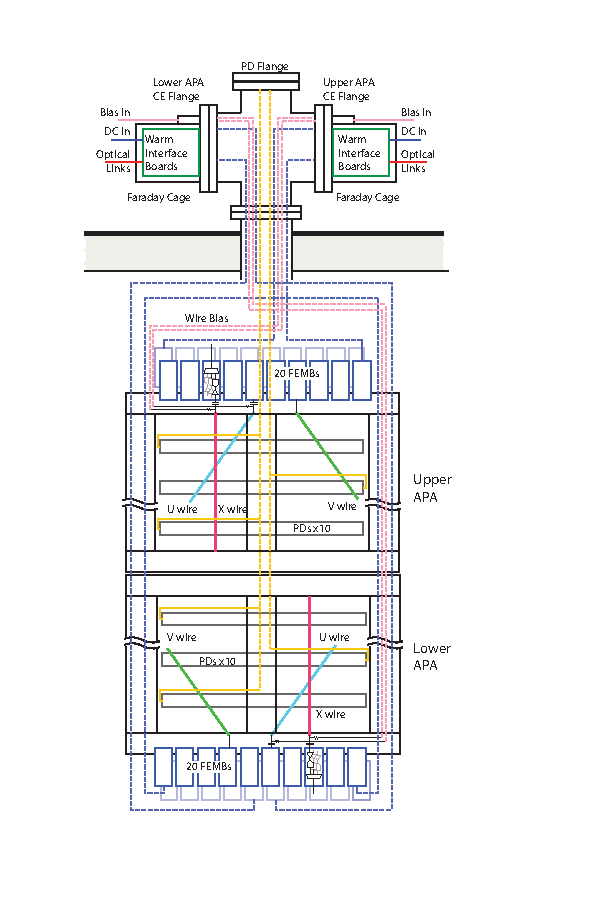
\includegraphics[width=0.7\textwidth]{sp-tpcelec-DUNE-FD-APA-readout-scheme-v1.pdf}
\end{dunefigure}

The baseline design for the \dword{spmod} \dword{tpc} electronics (the \dword{ce}) calls for three 
types of custom \dwords{asic} inside  the \dword{lar}:
\begin{itemize}
\item{a \num{16}-channel \dword{fe} \dword{asic} for amplification 
and pulse shaping (referred to as \dword{larasic});}
\item{a \num{16}-channel \num{12}-bit \dword{adc} \dword{asic} 
operating at \SI{{\sim}2}{MHz}; and}
\item{a \num{64}-channel control and communications \dword{asic} 
(referred to as \dword{coldata}).}
\end{itemize}

%The complete list of 
The \dword{ce} components %of the  
required for one \dword{apa} are: 
\begin{itemize}
\item{\dwords{femb}, on which the \dwords{asic} are mounted, and 
which are installed on the \dword{apa}s;}
\item{cables for the data, clock, and control signals; \dword{lv} 
power; and wire bias voltages between the \dword{apa} and the 
signal flanges (cold cables);}
\item{signal flanges with a \dword{ce} \fdth to pass the data, clock, 
and control signals; \dword{lv} power; and \dword{apa} wire bias 
voltages between the inside and outside of the cryostat; and 
the corresponding cryostat penetrations and spool pieces;}
\item{\dwords{wiec} mounted on the signal flanges %and 
that contain
the \dwords{wib} and \dword{ptc}s for further processing
and distribution of the signals entering and exiting the cryostat;}
\item{cables for \dword{lv} power and wire bias voltages between 
the signal flange and external power supplies (warm cables); and}
\item{\dword{lv} power supplies for the \dword{ce} and bias-voltage 
power supplies for the \dword{apa}s.}
\end{itemize}

The number of channels (wires) connected to each of these
components is given in Table~\ref{tab:elecNums}.

\begin{dunetable}
[TPC electronics components and quantities for a single APA of a \dword{spmod}.] % dword for apa made this too long
{llr}
{tab:elecNums}
{TPC electronics components and quantities for a single \dword{apa} of the DUNE \dword{spmod}.}
\textbf{Element} &\textbf{Quantity} & \textbf{Channels per element}\\ \toprowrule
Front-end mother board (\dword{femb}) & \num{20} per \dword{apa} & \num{128} \\ \colhline
FE \dword{asic} chip & \num{8} per \dword{femb} & \num{16} \\ \colhline
\dword{adc} \dword{asic} chip & \num{8} per \dword{femb} & \num{16} \\ \colhline
\dword{coldata} \dword{asic} chip & \num{2} per \dword{femb} & \num{64} \\ \colhline
Cold cable bundle & \num{1} per \dword{femb} & \num{128} \\ \colhline
Signal flange & \num{1} per \dword{apa} & \num{2560} \\ \colhline
\dword{ce} \fdth & \num{1} per \dword{apa} pair & \num{2560} \\ \colhline
Warm interface board (\dword{wib}) & \num{5} per \dword{apa} & \num{512} \\ \colhline
Warm interface electronics crate (\dword{wiec}) & \num{1} per \dword{apa} & \num{2560} \\ \colhline
Power and timing card (\dword{ptc}) & \num{1} per \dword{apa} & \num{2560} \\ \colhline
\end{dunetable}

%The 
Successful operation of the readout electronics in \dword{lar} for the 
\dunelifetime %lifetime of the  (dunelifetime has ``years'' not ``year'')
of \dword{dune} operation %experiment forces 
imposes technological choices %that have to be implemented in the design of 
for the \dword{spmod} \dwords{asic},  % planned for the \dword{spmod}. It also imposes 
and specific constraints on commercial components that are installed
inside the \dword{lar}. While the higher charge carrier 
mobility~\cite{Hairapetian1989} at \dword{lar} temperature than at room
temperature is central to improving the performance of the  \dword{ce}, it also leads
to the hot carrier effect~\cite{Hot-electron}. 

In n-type \dword{cmos} transistors, the carriers (electrons)
can acquire enough kinetic energy to ionize silicon in the active channel. This
charge can become trapped and lead to effects (including threshold shifts)
similar to those caused by radiation damage, i.e., %. This effect 
can cause \dword{cmos}
circuits to age much more quickly at \dword{lar} temperature, %than at room temperature,
reducing performance and potentially causing failure. To mitigate this effect,
the maximum \efield in transistor channels must be lower than % the field 
that which could %can 
be used reliably at room temperature. 
\fixme{orig: This is accomplished by using transistors
fabricated with channel lengths that are larger than the length commonly used
for \dwords{asic} using the same technology, and operated at reduced bias voltage.}
%
This is accomplished by designing \dwords{asic} to use transistors 
with  channels two to three times longer than would be used at room temperature
and operating them at reduced bias voltage. 
%
We must carefully test any commercial circuits used in the \dword{lar} %must be carefully tested 
to ensure 
they will perform well for the expected experiment lifetime. %\dunelifetime lifetime of \dword{dune}; 
Reliability studies for \dword{fe} electronics designs under %in 
consideration are 
discussed in Section~\ref{sec:fdsp-tpcelec-qa-reliability}.

\dword{bnl} has been developing custom \dwords{asic} for \dword{lartpc} readout %has been going on at  
for many years, and %prototypes of 
\dword{larasic} prototypes have been used in previous \dwords{lartpc}, 
including the \dword{35t}, \dword{microboone}, and \dword{pdsp}. \dword{pdsp} is the first
experiment for which the charge digitization %of the charge 
and the data serialization
have been performed inside the \dword{lar}, using the P1-\dword{adc} \dword{asic} 
developed at \dword{bnl}. % and 
It also used a \dword{fpga} since \dword{coldata} was
still under development. %Further developments of \dwords{asic} for the \dword{dune} \dword{spmod} are discussed later in 
Section~\ref{sec:fdsp-tpcelec-design-femb} discusses further \dword{asic} developments for the \dword{spmod}.

%%%%%%%%%%%%%%%%%%%%%%%%%%%%%%%%%%%
\subsection{ProtoDUNE-SP Results}
\label{sec:fdsp-tpcelec-overview-pdune}

The \dword{pdsp}% \dword{protodune}-\dword{sp} 
detector, described 
in Chapter~\ref{ch:sp-execsum}, is a 700~ton fiducial volume 
\dword{lartpc} with 15,360 sense wires. 
The system was deployed in a beamline at the CERN Neutrino Platform 
in 2018 and continues to take cosmic event data into 2019. The goal of 
the \dword{pdsp} \dword{tpc} readout was to validate the concept 
and the design of the integrated \dword{apa}+\dword{ce} readout 
and measure the performance of the \dword{ce} system with components 
as close as possible to those in the final \dword{dune} \dword{tpc} readout.

Each of the six \dword{pdsp} \dword{apa}+\dword{ce}
readout units consists of 2,560 sense wires, of which 960 are \SI{6}{m} 
long collection wires and 1,600 are \SI{7.4}{m} long induction wires. 
Five of the six \dword{apa}s were tested in a full-scale cold box in 
cold gaseous nitrogen (GN$_2$) with a complete \dword{ce} readout system,  
identical to the one %on the detector, 
deployed in \dword{pdsp}, before installation in the cryostat,
while the sixth %one
 was installed without first going through the cold
box testing. Figure~\ref{fig:apa2-cycle} shows the measured noise, in 
electrons, for the collection (X) plane and the two induction (V, U) 
planes as well as the \dword{femb} temperature in the cold box as a 
function of the cold cycle time. At a stable temperature of 
\SI{160}{K} the noise for all three wire planes is less than 500~e$^-$.

\begin{dunefigure}
[\dword{pdsp} APA \#2 noise levels measured in GN$_2$ in the CERN cold box]
{fig:apa2-cycle}
{Left $y$ axis: Noise (in electrons) for U, V, and X (red, blue, and green 
curves) sense wire planes as a function of time (hours) for the APA \#2 cold 
cycle in GN$_2$ in the CERN cold box; right $y$ axis: temperature 
(orange curve) measured at the level of the \dword{fe} electronics.}
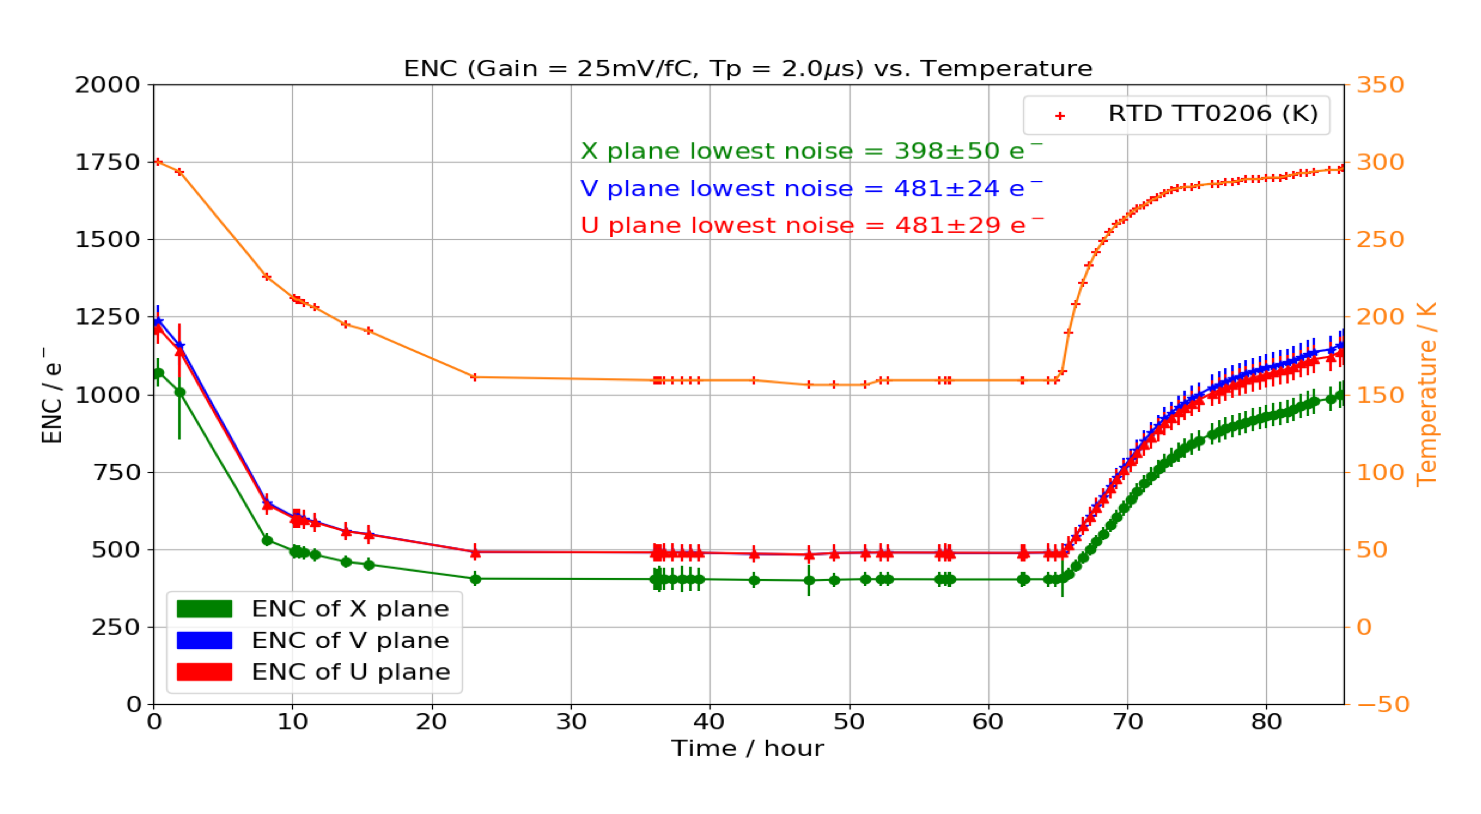
\includegraphics[width=0.95\linewidth]{sp-tpcelec-apa2.png}
\end{dunefigure}
%%% AH to here EOB 2/11
After the cryostat was filled with \dword{lar} and the drift and wire 
bias voltages were set to their nominal values (defined in Chapter~\ref{ch:sp-execsum}), 
99.7\% of the \dword{tpc} readout channels were live. % alive. 
The following 
channels were expected to be unresponsive %to charge deposited on the wires
based on tests performed prior to the insertion of the \dword{apa} into
the cryostat:
\begin{itemize}
\item{Four electronics channels, suggesting a dead channel in the electronics, 
all on collection wires, on three different \dword{apa}s;}
\item{ %14 channels measured with consistent with no capacitive load
Fourteen channels that consistently showed no capacitive load  
on the \dword{fe} electronics, suggesting an open connection somewhere upstream %in front 
of the \dword{ce} system, scattered randomly throughout the detector, 
and on all wire planes.}
\end{itemize}

\begin{comment}  No need for itemizing here (anne)
Two additional sets of channels were observed to be non-responsive
after filling the detector with \lar:
\begin{itemize}
\item{An additional 18 channels were found to be non-responsive
immediately after the \lar filling was complete;}
\item{Two more channels became non-responsive after the cathode
high voltage was raised to \SI{120}{kV}, and two more
when the high voltage reached \SI{180}{kV}.}
\end{itemize}
\end{comment}
After filling the detector with \lar{}, an additional 18 channels stopped responding. Two more  followed  after the cathode \dword{hv} was raised to \SI{120}{kV}, and another two when the \dword{hv}  reached \SI{180}{kV}.



No %There hasn't been any 
further loss of readout channels has occurred since 
the end of September 2018.
With the detector operating under nominal %operating 
conditions, the noise
measured by the online monitoring program was approximately 550~e$^-$ 
on the collection wires and approximately 700~e$^-$ on the induction
wires, averaged over all operational channels. The noise increased %s
relative to the tests performed inside the cold box due to the 
larger dielectric constant of \lntwo 
\fixme{not \lar{}?} relative to GN$_2$. 
These noise measurements  %in the two conditions 
are consistent with the 
ratio of the corresponding capacitances of the \dword{apa} wires. 
Figure~\ref{fig:apa3-noise} 
shows the noise (in electrons) for all channels of one %of the 
\dword{apa}+\dword{ce} readout unit. %s. 
The collection channels with noise larger than \SI{1500}{e$^-$} had a problem %are caused by a problem
 in the P1-\dword{adc} 
\dword{asic};  %used in \dword{protodune}-\dword{sp},
this problem had already
been identified %at the time of testing the components 
prior to their
installation on the \dwords{femb}. The channels on all three planes 
with noise smaller than \SI{300}{e$^-$} have an open connection somewhere in 
front of the \dword{ce} system. Figure~\ref{fig:ENC-all} summarizes
noise levels in the entire \dword{pdsp} detector both before and
after the application of a simple common-mode filter; an improvement
of roughly 100~e$^-$ is seen on all planes. % after the common-mode filter is applied.

\begin{dunefigure}
[TPC noise levels measured at \dword{pdsp} after \lar fill]
{fig:apa3-noise}
{Noise (in electrons) for all U, V, and X (red, blue, and green curves) sense 
wire planes for one \dword{pdsp} \dword{apa} %with the detector in 
under nominal operating 
conditions.}
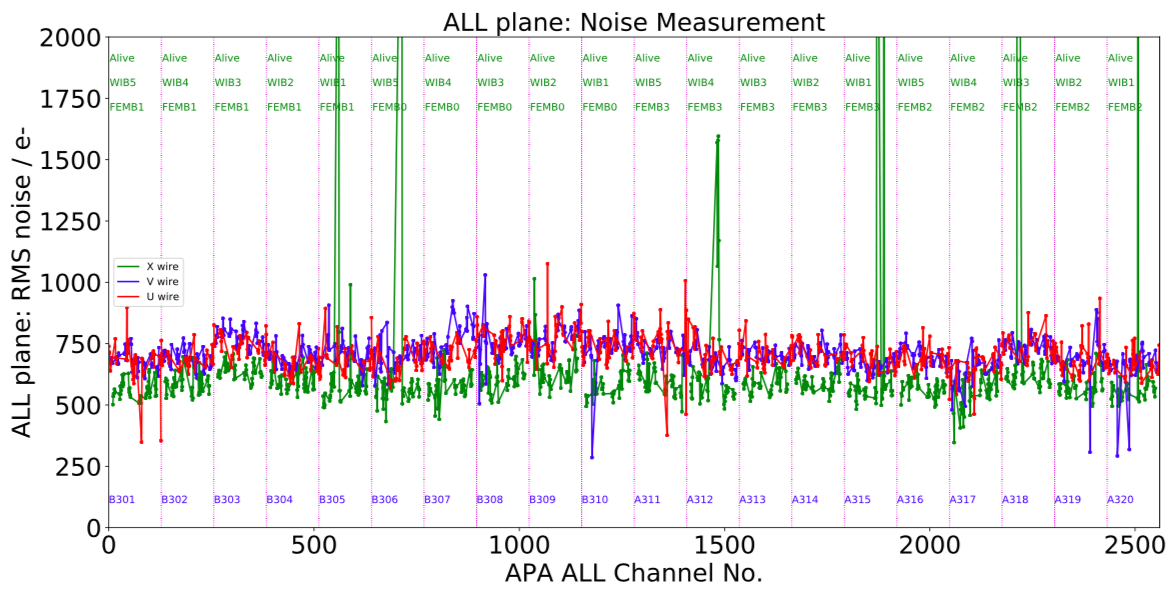
\includegraphics[width=0.9\linewidth]{sp-tpcelec-apa3-enc.png}
\end{dunefigure}

\begin{dunefigure}
[\dword{tpc} noise levels for all channels of the \dword{pdsp} detector]
{fig:ENC-all}
{Noise levels (in \dword{enc}) for all channels of the \dword{pdsp} detector, both
before and after the application of a simple common-mode filter.}
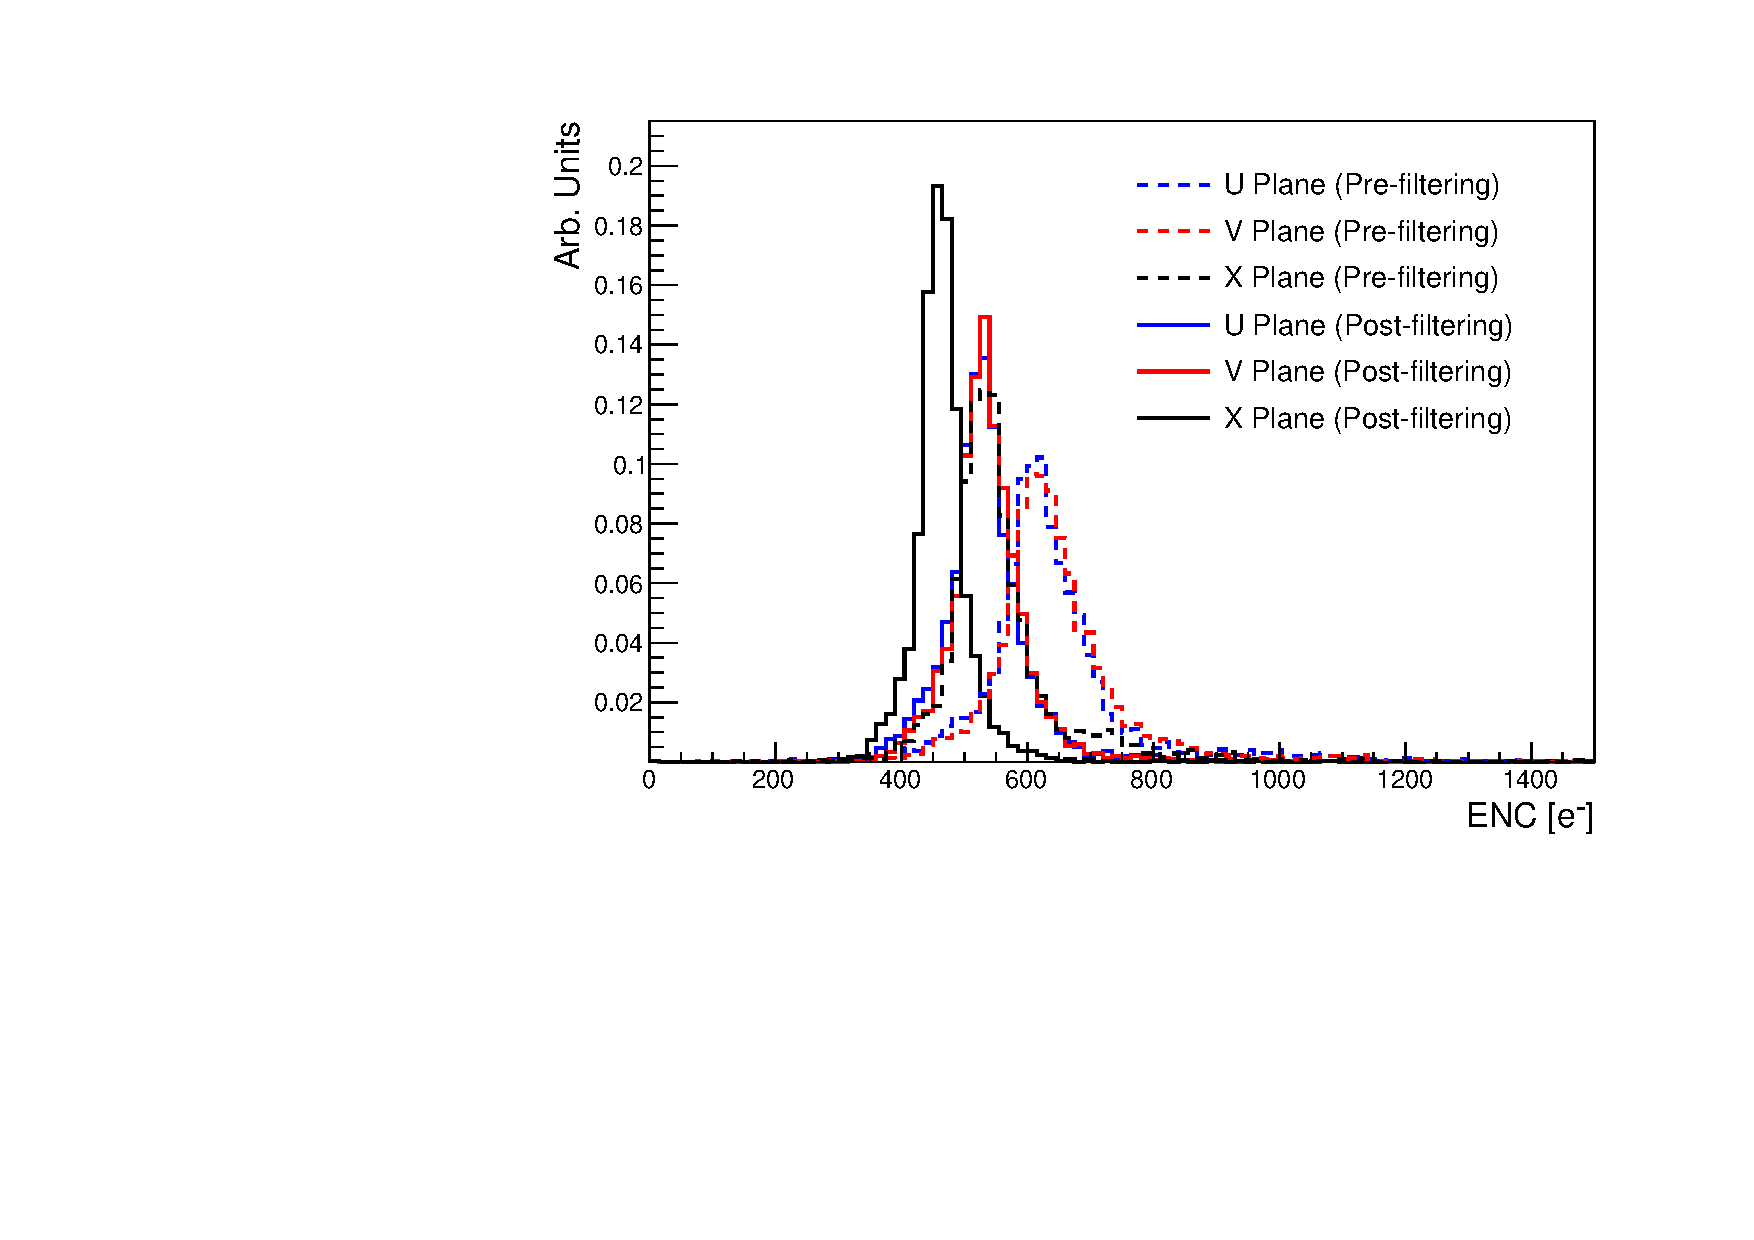
\includegraphics[width=0.65\linewidth]{sp-tpcelec-ENC-Combined.pdf}
\end{dunefigure}

The overall performance of the \dword{ce} system in 
\dword{pdsp} satisfies the %\dword{dune} \dword{sp} \dword{fd} 
\dword{ce} system specifications %requirements 
for the \dword{spmod} %\dword{fd} 
listed in Section~\ref{sec:fdsp-tpcelec-overview-requirements}. 
%Another demonstration of the performance achieved
%and of the progress made since previous detectors based on the
%\dword{lartpc} technology is given by 
%
A comparison of the raw data from 
a \dword{pdsp} event (Figure~\ref{fig:pdsp-display}) to 
that from a \dword{microboone} event (Figure~\ref{fig:microboone-display}~\cite{Acciarri:2017sde}) demonstrates the improvements achieved in \dwords{lartpc} performance. 
The \dword{pdsp} event was collected very early in the data taking
period when the charge collection efficiency was still limited
by the amount of impurities in the \dword{lar}; it shows very little
noise and appears to be of the same quality as the \dword{microboone}
event display after offline noise removal. 
% This clearly demonstrates %shows -- repetitive (anne)
%that significant progress has been made 
%significant progress in the overall system
%design,  % based on the lessons learned from previous experiments
%using the \dword{lartpc} technology, 
%resulting in immediate collection of high quality
%data with very little noise. % immediately after the beginning of data taking.

\fixme{Marco: the ProtoDUNE event display will be replaced (same event, 
but view before removal of common-mode noise).}

\begin{dunefigure}
[Raw data from a \dword{pdsp} event]
{fig:pdsp-display}
{Display of the charge deposited on the collection wires ($x$-axis) as
a function of the drift time ($y$-axis) for a \dword{pdsp} event 
that includes two electromagnetic showers and a four-prong interaction.
The color associated with each time sample on the \dword{apa}
wires gives a measurement of the charge measured by the \dword{ce}
readout, increasing from the smallest values (blue) to the largest
ones (red).}
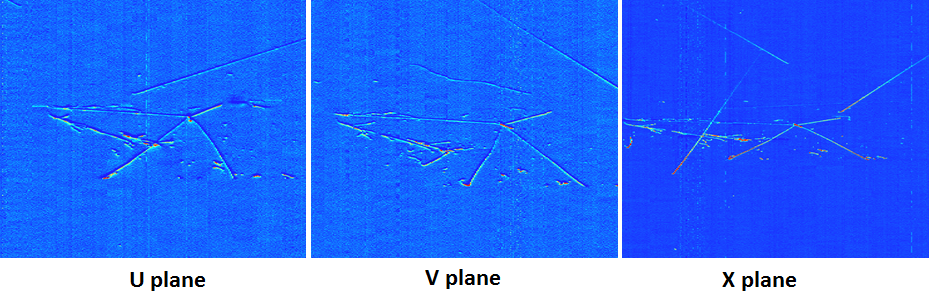
\includegraphics[width=1.0\linewidth]{sp-tpcelec-4prongdisplay.png}
\end{dunefigure}

\begin{dunefigure}
[Raw data from a \dword{microboone} event]
{fig:microboone-display}
{\dword{microboone} \twod event display of the V plane from run 3493 
event 41075 showing the raw signal (a) before and (b) after offline 
noise filtering. A clean event signature is recovered once all the 
identified noise sources are subtracted~\cite{Acciarri:2017sde}.}
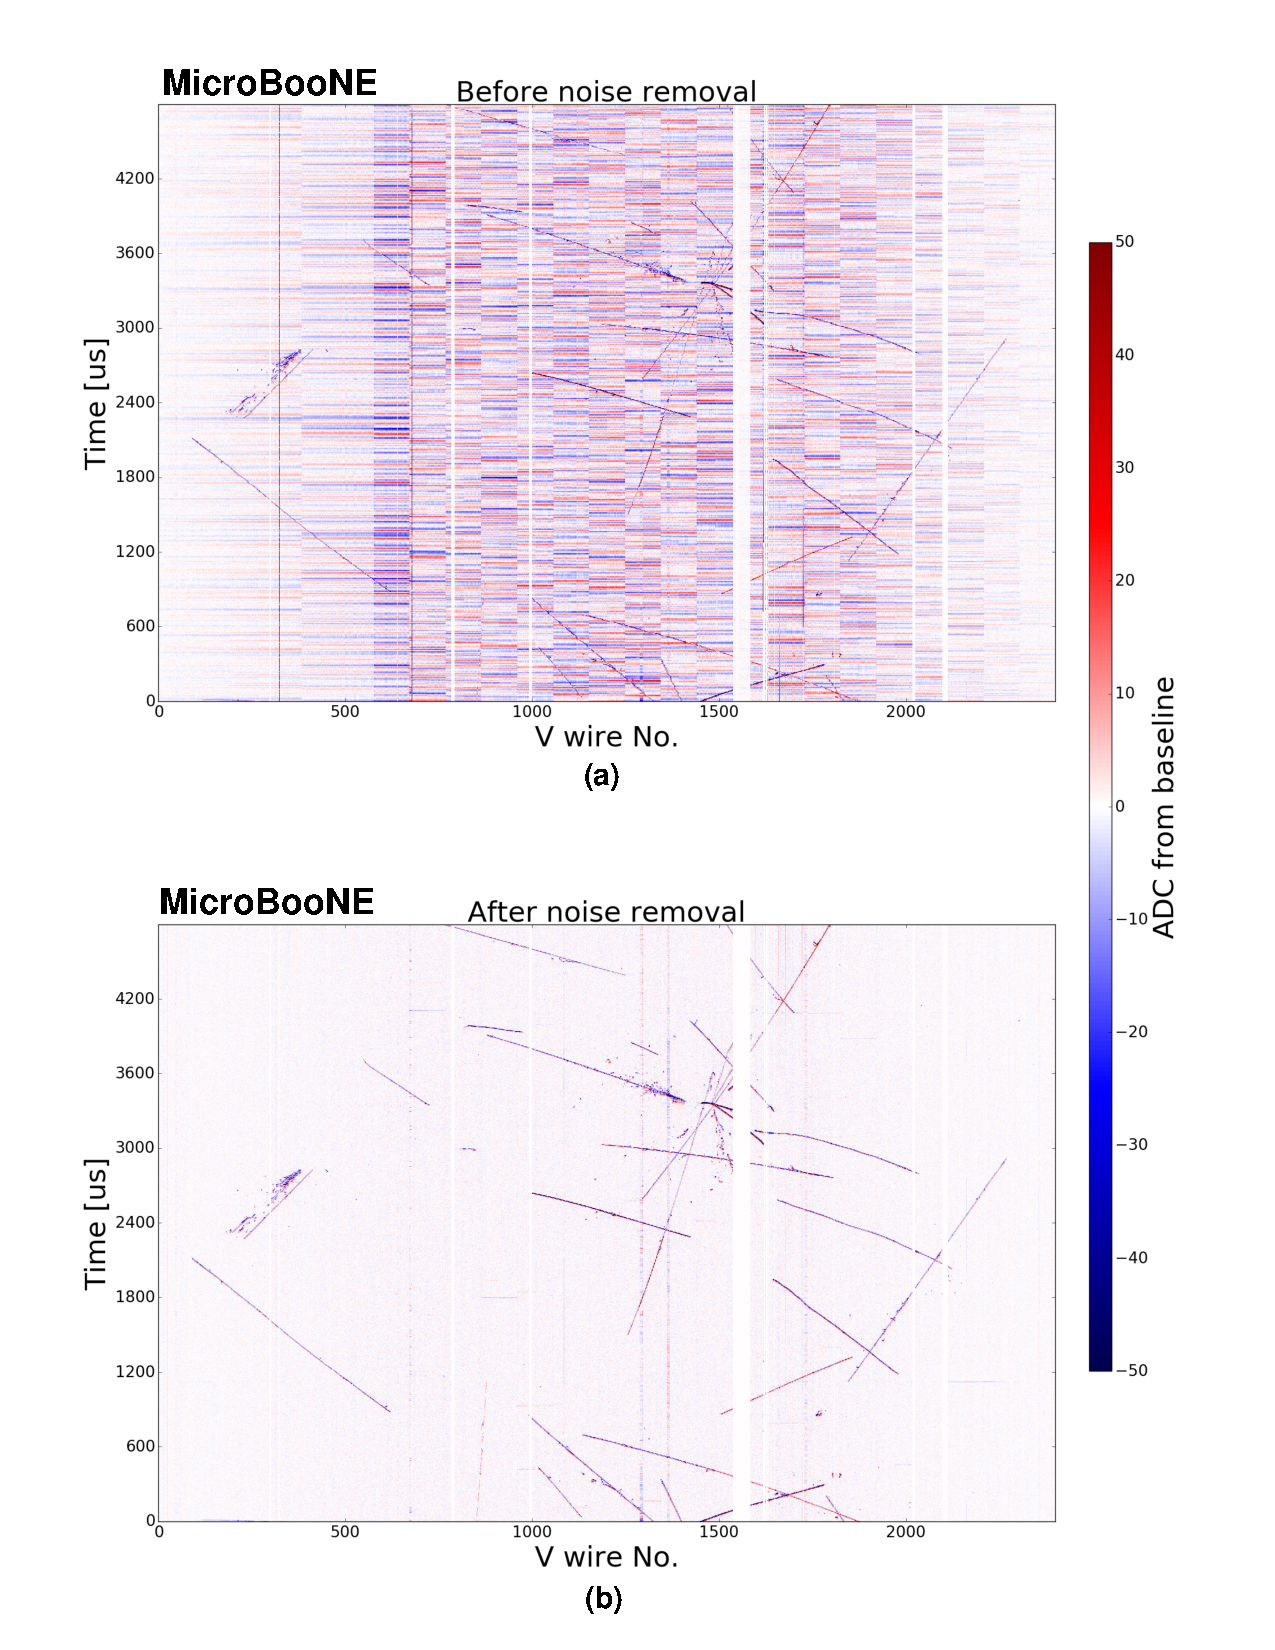
\includegraphics[width=0.9\linewidth]{microBoone_display.pdf}
\end{dunefigure}

%%%%%%%%%%%%%%%%%%%%%%%%%%%%%%%%%%%
\subsection{ProtoDUNE-SP Lessons Learned}
\label{sec:fdsp-tpcelec-overview-lessons}

As discussed in %the previous 
Section~\ref{sec:fdsp-tpcelec-overview-pdune}, the initial data from \dword{pdsp}
show that the \dword{spmod} %dune} detector 
can meet the  %requirements 
specifications. % presented in Section~\ref{sec:fdsp-tpcelec-overview-requirements}. % can be met.
The experience with the \dword{ce} in \dword{pdsp} nonetheless motivates several improvements %and updates 
to the \dword{ce} system design.  %are motivated by. 
%results of the testing, %and 
%commissioning, and operation of %, and the data-taking with, 
%the \dword{pdsp} electronics. 
A complete list of the lessons learned from the construction, testing, integration,
installation, commissioning of the \dword{ce} detector components
is available~\cite{bib:docdb12367}. This reference also discusses %In addition to reporting the lessons learned, 
the plans and timeline for addressing the issues 
observed in \dword{pdsp}. % are also discussed in this document. Here
This \dword{tdr} section and the following cover only the main issues  % are discussed, 
and the plans for their resolution  
%are discussed in the next Section, where the planned design changes
for implementation in the \dword{spmod}. %\dword{dune} detector are discussed.

The main problem with the \dword{pdsp} \dword{ce} readout is in the
P1-\dword{adc} \dword{asic}. This problem was observed as early as 2017 %already in 2017
while these \dwords{asic} were being tested prior to their installation
on the \dwords{femb}. % The main issue with the P1-\dword{adc} is that the
The ``domino'' architecture used in this design relies on
excellent transistor matching, which %and 
unfortunately %transistor matching
is worse at \dword{lar} temperature. In \dword{pdsp} this problem
results in some readout channels having a fixed value for some of
the \dword{adc} bits. Some of these channels need to be masked 
from analysis, resulting in a loss of efficiency for \dword{pdsp}, while
in a majority of cases an approximated value for the charge can
be obtained via interpolation. 
\fixme{some of the ``some channels'' needed masking? An approx value was obtained for a majority of the ``some channels'' (not the masked ones?) } 
%Due to this problem, plans have been put  in place to develop an \dword{adc} with a completely new design for the \dword{dune}. 

To resolve this problem, a  \dword{bnl}-\dword{fermilab}-\dword{lbnl} collaboration is developing a new \dword{adc} \dword{asic} (called a 
\dword{coldadc} \dword{asic}), and first
prototypes are planned to be characterized in February 2019. %The design
%of this \dword{adc} is discussed in detail in 
Section~\ref{sec:fdsp-tpcelec-design-femb-adc} presents a detailed design.  In parallel, two
alternatives are being considered. %for  \dword{dune}. 
First, the \dword{sbnd} 
collaboration has found %demonstrated that there is also 
a \dword{cots} 
solution for the analog-to-digital conversion, based on the Analog 
Devices~\cite{AnalogDevices} AD7274~\cite{AD7274} \dword{adc}, that meets 
the \dword{dune} specifications %requirements 
and that could be used in the \dword{spmod} in %the
case  the custom \dword{asic} is not %developments were not successfully
completed in time. % for the detector construction. 
This \dword{cots}
solution is not the preferred approach for \dword{dune} since it
requires one \dword{asic} for each readout channel (i.e., a total
of \num{384000} chips), which would increase the cost %cause significant cost increases
and %would 
require a very extensive \dword{qc} program. The qualification
of this \dword{cots} \dword{adc} for use in \dword{dune} is described
in Section~\ref{sec:fdsp-tpcelec-design-femb-alt-cots}. 
The second alternative is a single \num{64}-channel \dword{asic}, referred to as a \dword{cryo},
that consolidates the \dword{fe}, the analog-to-digital conversion, and the
data serialization functions %alities 
in a single chip. %This  development 
It has also reached the prototype stage with \dword{asic} %that are planned to be 
characterization planned in February 2019. %More details about this solution are discussed in 
Section~\ref{sec:fdsp-tpcelec-design-femb-alt-cryo} provides details.

Initial analysis of the \dword{pdsp} data has uncovered %shown 
a new problem 
with \dword{larasic} %The problem 
that occurs when %a large amount of change (
$>$\SI{50}{fC} is collected over a period of \SIrange{10}{50}{$\mu$s}.
%This causes 
The feedback mechanism of the \dword{fe} amplifier 
% to stop 
stops working for %a certain period of time (
several hundred $\mu$s.  %In 
During this period, the readout does not function %is not functioning 
and signals following 
the large charge deposited can %may 
be completely lost. A ledge is observed 
in the output of the \dword{fe} amplifier, followed by a slow decay 
and a sudden turn-on of the amplifier. %An example of this behavior from data is shown in 
Figure~\ref{fig:pdsp-ledge} shows an example of this behavior.

\begin{dunefigure}
[Pulse shape on a \dword{pdsp} wire showing the ledge effect]
{fig:pdsp-ledge}
{Waveform of an event showing the ledge following a large charge 
deposition, then a discharge and a final jump to the normal baseline.}
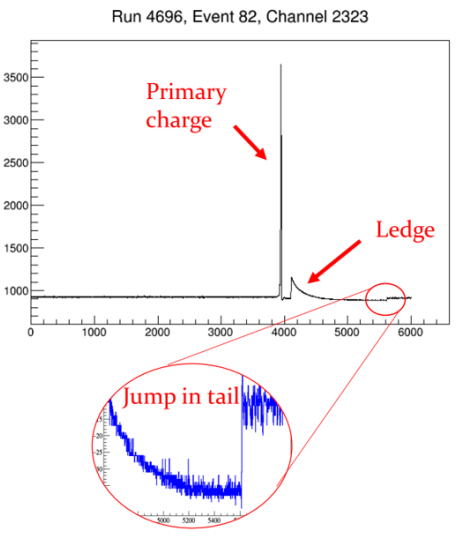
\includegraphics[width=1.0\linewidth]{sp-tpcelec-ledge.png}
\end{dunefigure}

This problem has been reproduced in the laboratory and is being actively 
studied. It affects all versions of \dword{larasic} fabricated after 
the one used for the \dword{microboone} experiment. The problem occurs 
with larger probability for the \SI{200}{mV} baseline used for the collection
wires than for the \SI{900}{mV} baseline used for the induction wires.
After the problem and this difference between the two baselines were 
observed, the decision was taken to operate the \dword{ce} in \dword{pdsp} 
using the \SI{900}{mV} baseline also for the collection wires, sacrificing
the dynamic range. Data from the wires where the problem occurs can
be masked in analysis, resulting in a loss of efficiency. It should be
noted that the problem occurs more often in \dword{pdsp} %compared to
%\dword{dune} 
than is expected in the \dword{fd}  \dword{spmod} due to the presence of cosmic rays traveling parallel
to the \dword{apa} wires. % in the first case. 
The problem %cannot be discounted for \dword{dune}, however, since it 
could, however, affect the \dword{spmod}'s ability to detect
electromagnetic showers -- one of the main physics signals.
%The plan and the timeline for addressing this issue in a new \dword{larasic} prototype
%of  are going to be discussed in 
Section~\ref{sec:fdsp-tpcelec-design-femb-fe} discusses the plans and timeline for addressing this issue in a new \dword{larasic} prototype.

\begin{dunefigure}
[Image of a connector for the cold cables lifted from the \dword{femb}]
{fig:pdsp-femb-connector}
{Image of a connector for the cold readout and signal cables lifted from
the \dword{femb} due to the presence of excess epoxy on the 
connection between the cold cables and the printed circuit board
that acts as the ``male'' part of the connector.}
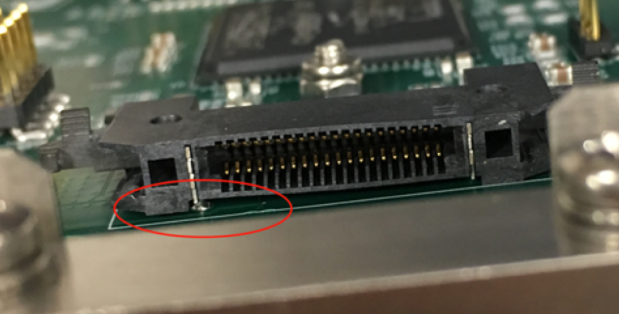
\includegraphics[width=1.0\linewidth]{sp-tpcelec-femb-problem.png}
\end{dunefigure}

\begin{comment}During the integration of the \dwords{femb} onto the \dword{apa}s 
and the cold tests that preceded the \dwords{apa} installation
inside the \dword{pdsp} cryostat a problem occurred %was observed 
on the 
connection between the cold readout and control cables and the
\dwords{femb}. In multiple cases the connector %is 
detached from
the \dword{femb} causing a loss of communication. 
\end{comment}
During the integration of the \dwords{femb} onto the \dword{apa}s 
and the cold tests that preceded the \dword{apa} installation
inside the \dword{pdsp} cryostat,  multiple connectors  
detached from
the \dword{femb}, causing a loss of communication.  
%For \dword{pdsp} w
We replaced the \dwords{femb} %This problem was fixed for 
on all the \dword{apa}s that had been tested in the cold box. % by replacing the \dword{femb}. 
One additional \dword{femb} was 
replaced on the \dword{apa} that had been installed without undergoing 
the test in the cold box. This %problem 
detachment may also be the cause
of the loss of the external clock signal on one of the \dwords{femb}
that was observed after cooldown. % of the detector. 
%
The problem 
with the connector has been traced to a mechanical interference between 
the epoxy deposited as a protective measure on the small printed circuit
board to which the cold cables are soldered and which forms the 
male part of the connector. The height of the epoxy can cause 
the female part of the connector to lift, % from, 
as shown in 
Figure~\ref{fig:pdsp-femb-connector}. %This problem is being 
%addressed by a redesign of the connection between the \dword{femb}
%and the cold cables, as discussed in 
Section~\ref{sec:fdsp-tpcelec-design-femb} discusses the redesign of the connection to address the problem.

\begin{dunefigure}
[Spectrum of the noise on the \dword{pdsp} \dword{apa} wires before and after noise filtering]
{fig:pdsp-noise}
{Spectrum of the noise on the different \dword{pdsp} \dword{apa} wire planes before
(left) and after (right) applying a simple common-mode filter.}
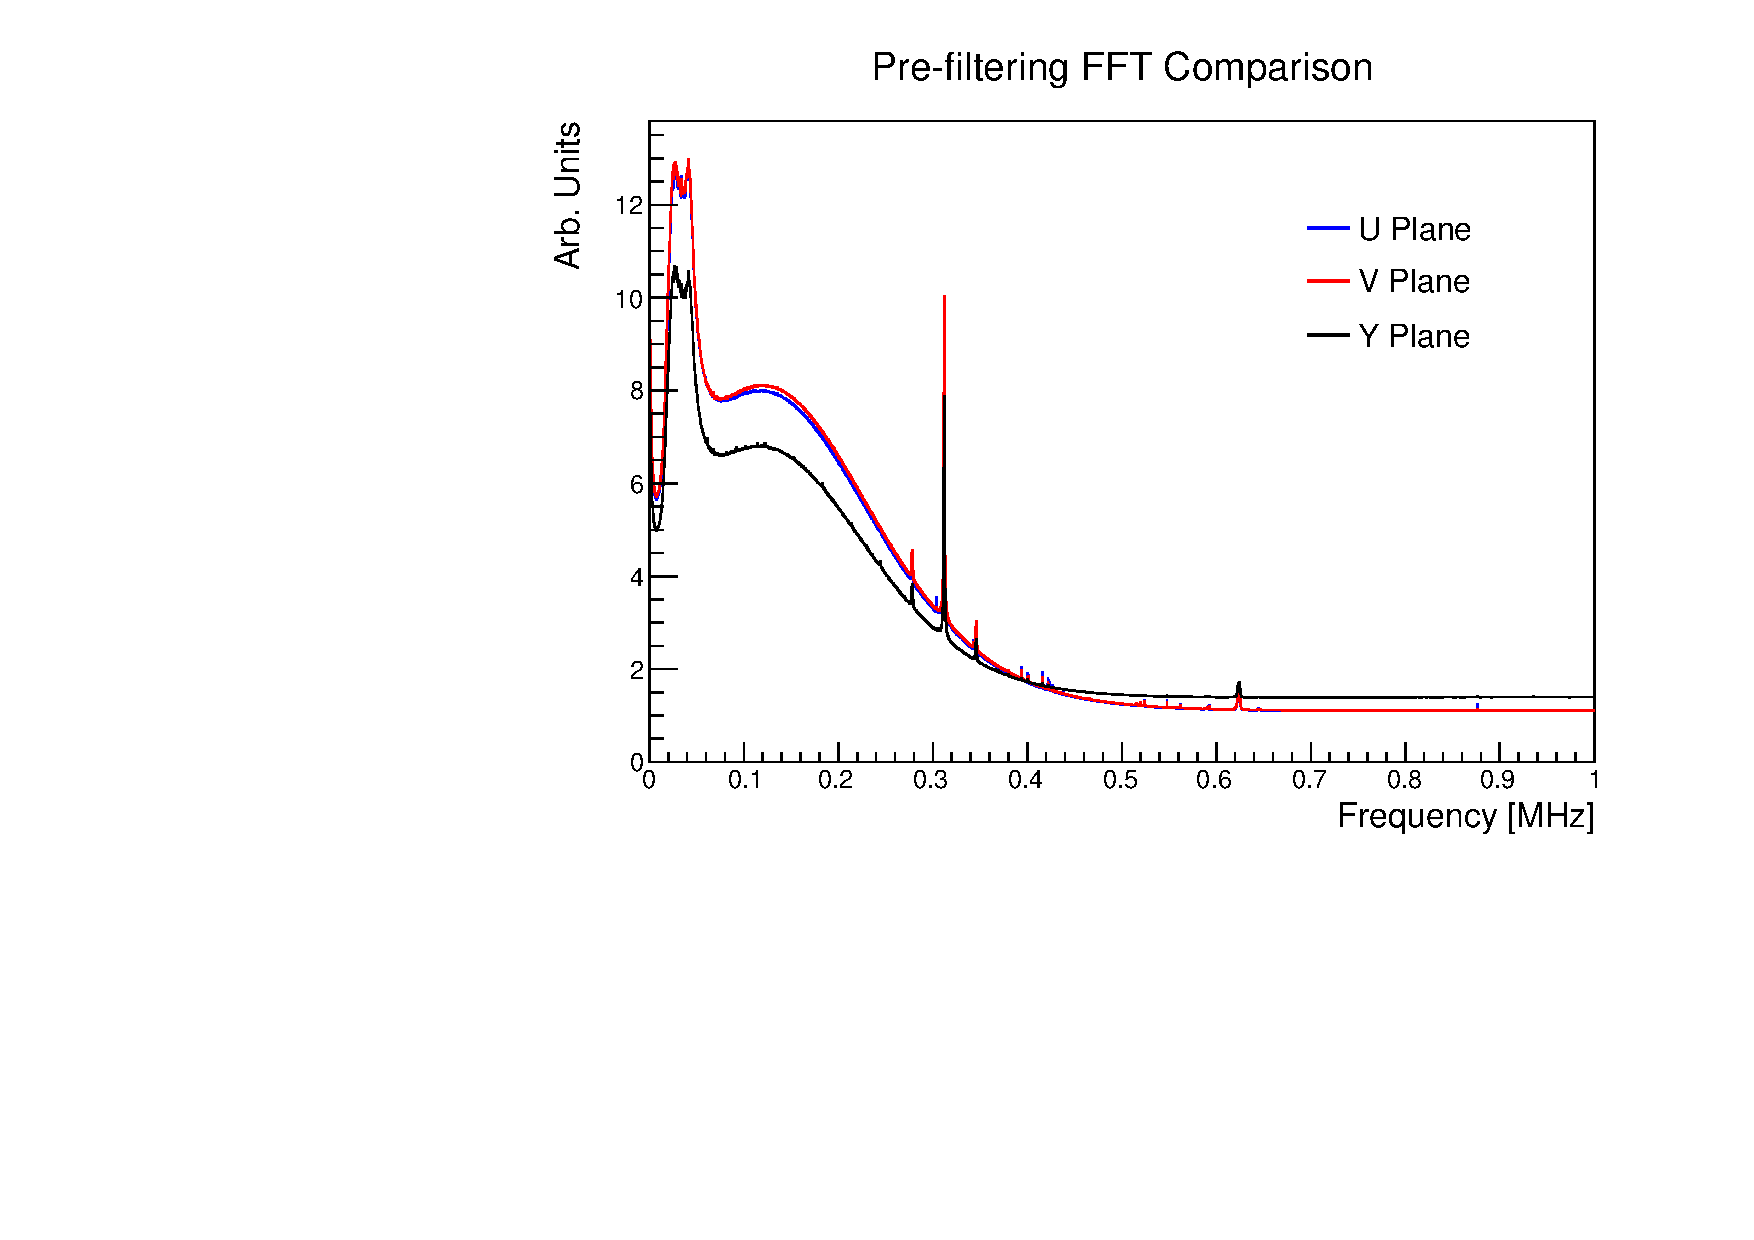
\includegraphics[width=0.49\linewidth]{sp-tpcelec-avgFFT-WithoutFilt.pdf}
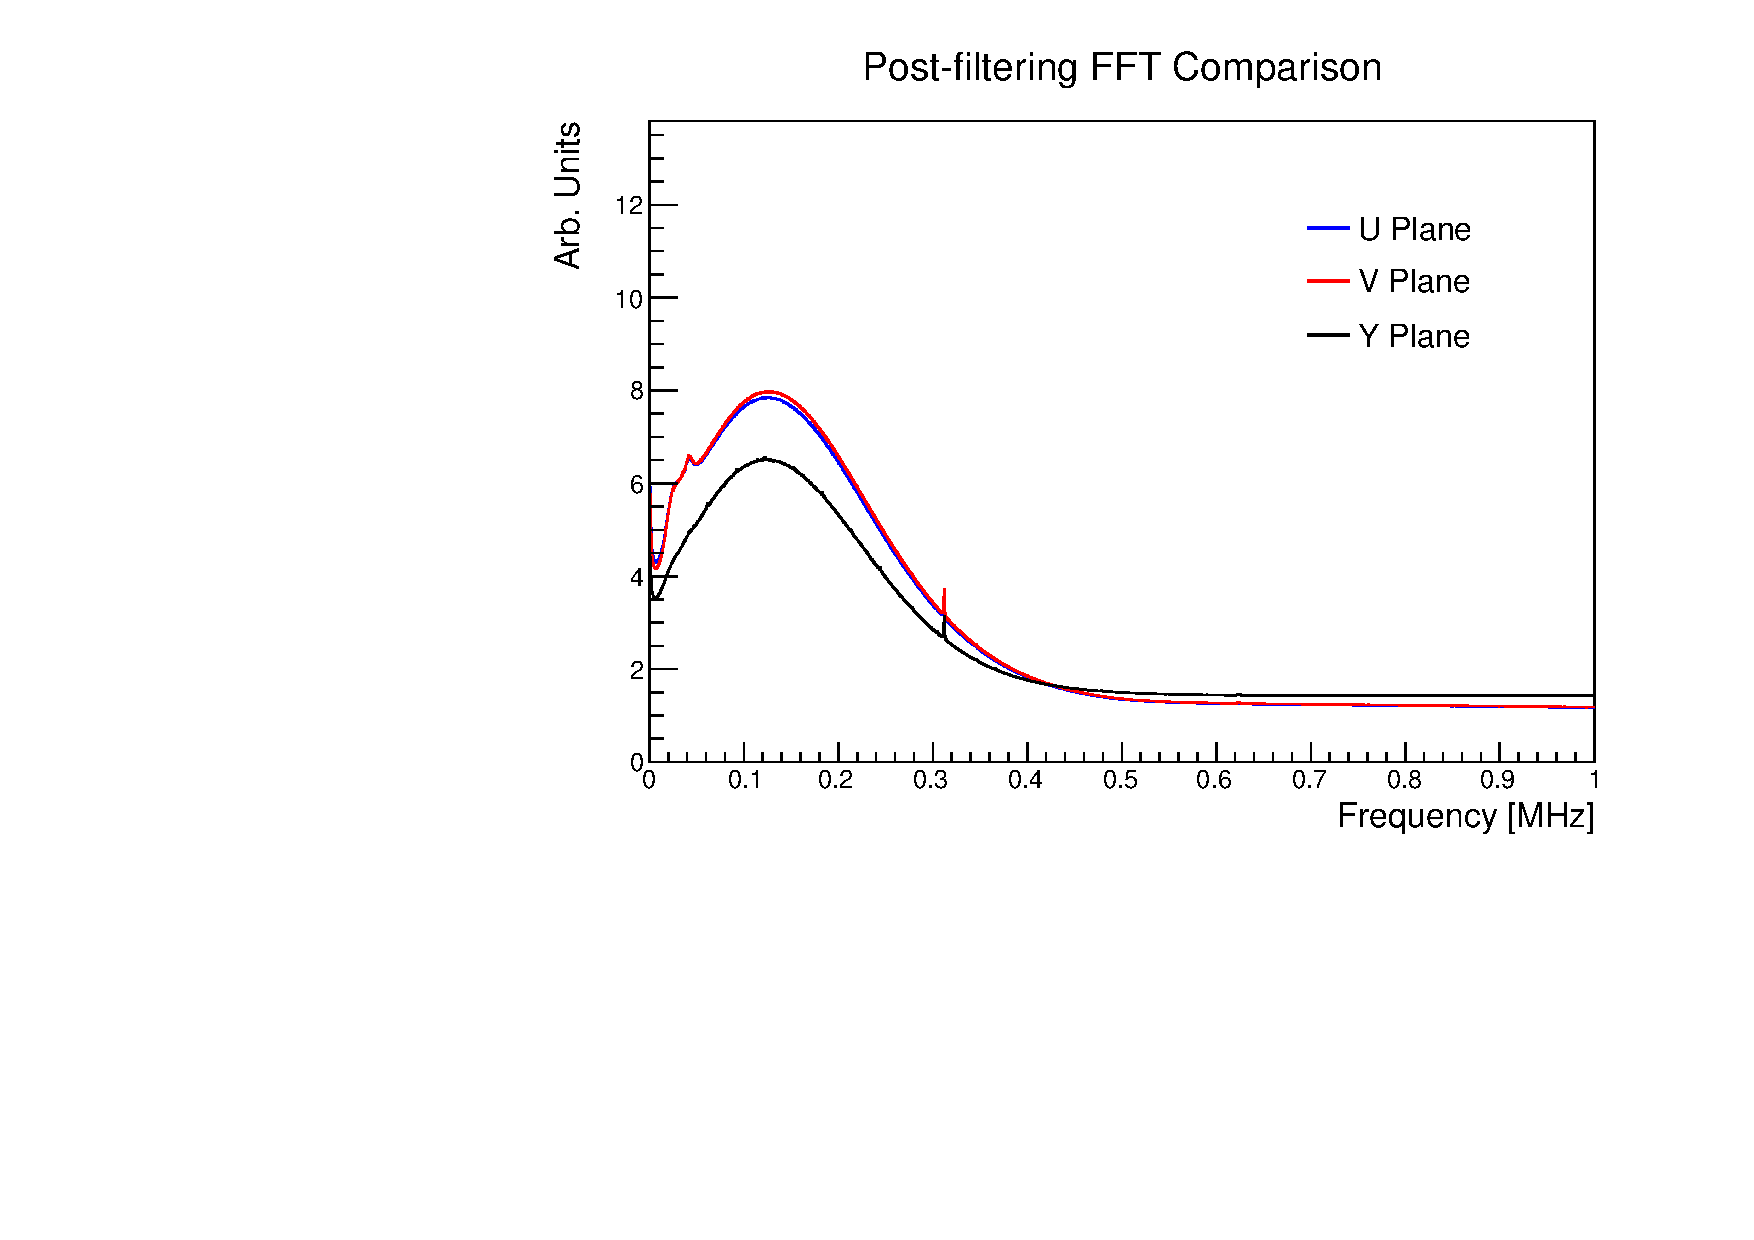
\includegraphics[width=0.49\linewidth]{sp-tpcelec-avgFFT-WithFilt.pdf}
\end{dunefigure}

%Finally, it should be noted that the 
Analysis of the \dword{pdsp} data
is just starting, as of February 2019, and %that there is a lot to learn about the
we will learn more about the detector and how its different components %of the detector 
interact %among themselves 
from this data. The level of noise mentioned in Section~\ref{sec:fdsp-tpcelec-overview-pdune}
%the previous section 
(approximately \SI{550}{e$^-$} on the collection wires,
and approximately \SI{700}{e$^-$} on the induction wires) 
was obtained from the online data monitoring, without any
filtering or selection applied to the pulses on the \dword{apa}
wires. A simple common-mode filter can significantly reduce the 
noise, particularly at low frequencies, as shown in Figure~\ref{fig:pdsp-noise},  
%,that contains 
a comparison of the noise spectrum on the three planes of the \dword{apa} before and after the filtering. 
The spectrum prior to
the filtering shows %some interesting features. At 
that at %very low
frequencies $<$\SI{60}{kHz}  the %noise is dominated by the
low-voltage regulators %that are 
installed on the \dwords{femb} dominate the noise.  
%The noise from the low voltage regulators 
This contribution to the noise has actually
been significantly reduced %in \dword{pdsp} 
compared to
initial observations at \dword{microboone}~\cite{Acciarri:2017sde},
thanks to hardware filters developed at \dword{microboone} that we have% been
added on the \dword{pdsp} \dwords{femb}. The noise spectrum prior to the
filtering also shows spikes at multiple discrete frequencies, and in
some cases the noise %spectrum 
sources have been identified (e.g., cameras,
malfunctioning bias voltage supplies). We expect that further data analysis
and %further 
tests with \dword{pdsp} %could result in further
will result in improvements to the %already excellent \dword{ce} performance
%and will be reflected, if appropriate, in changes of the
%detector design.
 \dword{ce} design that already demonstrates excellent performance.
